\documentclass[12pt,oneside]{article}
\newcommand{\name}{Jean-Yves Djamen}
\newcommand{\class}{Math 80266A}
\newcommand{\hwnumber}{3}

\usepackage[margin=1in,letterpaper]{geometry}
%geometry changes the margins
%inside straight bracket is a parameter, inside curly bracket is name of package or whatever
%

\usepackage{amssymb,amsthm,amsmath,enumerate,fancyhdr,graphicx,tabularx}
\usepackage{float}
\usepackage{microtype}
\usepackage{tikz}
%Enables Graph Theory
\usepackage{pgfplots}
\usepackage{mdframed}
\usepackage[T1]{fontenc}
%Draws fancy boxes
\usepackage{parskip}
%Paragraph skip
\linespread{1.1} 
%Space in between lines
\usepackage{sectsty}
\sectionfont{\fontsize{12}{15}\selectfont}

\newenvironment{problem}[1]
{\begin{mdframed}
%Frames and crap
        \textbf{\textsc{Problem #1:}}
}
{\end{mdframed}}


\newenvironment{solution}
    {\textbf{\textsc{Solution:}}\\}
    {\newpage}

\pgfplotsset{compat=1.16}
\pagestyle{fancy}
\lhead{\textbf{\name}}
\chead{}
\rhead{\textbf{\class\ Assignment\ \hwnumber}}
\rfoot{\thepage}
\cfoot{}
\renewcommand{\headrulewidth}{0.2pt}

%lhead is the left header
%/textbf is text bold header

\def\l{\ell}
\def\pt{\partial}
\def\fish{\mathcal{I}}
\begin{document}

% \begin{enumerate}[I.]
% \item Solution number 1
% \item Solution Dos
% \item 
% \end{enumerate}

%/includgraphics

%/begin{align*}
%Stuff in here
%If star isn't included then the align command will automatically number your crap
%/end{align*}


\begin{problem}{1}
Simulate 1000 observations from each of the following data models. In each case, construct a Hill plot and comment.
\begin{enumerate}
    \item Consider an iid sequence with standard Cauchy marginal df.
    \item  Consider an iid sequence with standard Normal marginal df.
    \item Consider an AR(1) process $X_t = \phi X_{t-1} + Z_t$ where $\phi \in \{0.9, 0.5, 0.2\}$ and the noise sequence $\{Z_t\}$ comes from a symmetric distribution with exact Pareto tail $P(Z > x) =0.5x^{-10}$, $x \geq 1$. This yields $P(X > x) \sim cx^{-10}$.
\end{enumerate}
\end{problem}

\begin{solution}
We look now at several hill plots. Our goal is to notice a region of stability; preferably around small order statistics.
\section{Standard Cauchy}

We observe a region of stability around 1 which suggests the cauchy distribution has a tail index of 1.
\begin{figure}[H]
\begin{center}
{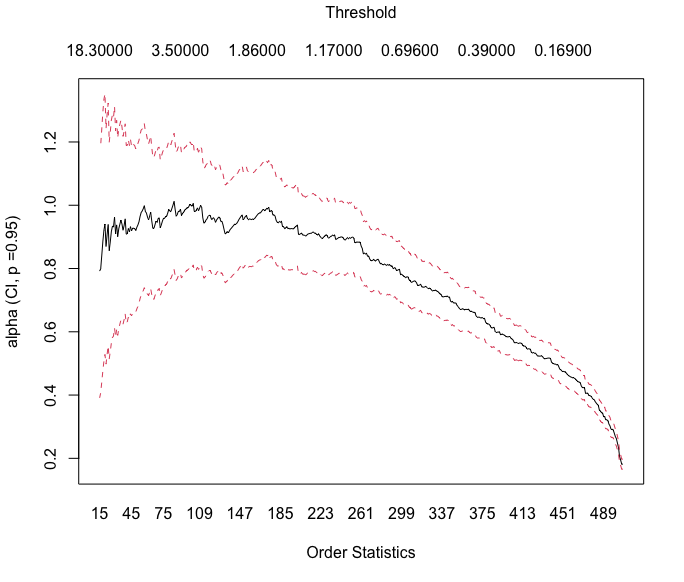
\includegraphics[width=3in]{Assignments/a3/hill-plot-cauchy.png}}
\caption{Hill plot for standard Cauchy distribution.}
\end{center}
\end{figure}

\section{Standard Normal}
Due to the intractability of the erf function, we expect condition (2) to not be completely satisfied, thus yielding an erratic and non-interpretable Hill plot.
\begin{figure}[H]
\begin{center}
{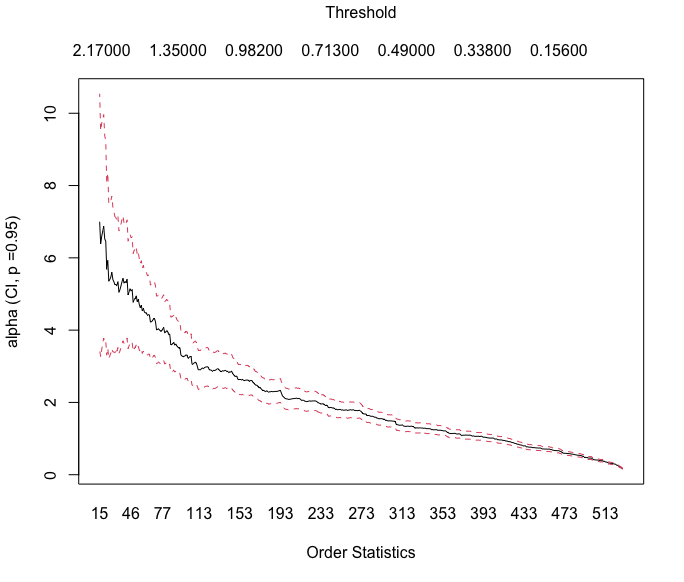
\includegraphics[width=3in]{Assignments/a3/hill-plot-normal.png}}
\caption{Hill plot for standard Normal distribution.}
\end{center}
\end{figure}

\section{AR(1) Processes}
First, we must recover the density function of the noise variable $Z_t$. Given that the sequence $\{Z_t\}$ is a symmetric distribution to be used as noise in an AR(1) process, as well as the right-sided behavior, we can sample points from $Z$.
\[P[Z\leq x] =\begin{cases} 1-0.5x^{-10} & x \geq 1 \\
0.5x^{-10} & x \leq -1 \end{cases}\]
Note that as $\{Z_t\}$ is to be used as a noise variable for an AR process, ensure that our cdf is symmetric around 0 and has an expectation of 0. Furthermore, we can invert the CDF and use uniform draws from (0,1) to sample from this sequence:
\[x=\begin{cases} [2(1-p)]^{\frac{-1}{10}} & \frac{1}{2}< p\leq 1\\
-([2p]^{\frac{-1}{10}}) & 0<p\leq \frac{1}{2}\end{cases}\]
Additionally, we are given that any AR(1) process we fit with this noise will have
\[P(X>x)\approx cx^{-10}\]
So, in the graphs below, we would hope to see a region of stability around $\hat{\alpha}=10$. However, the convergence of the Hill estimator hinges on the dependence of the sequence. We expect to see poor results for $\phi=0.9,0.5$ as the dependence between elements in these sequences can in no way be defined as ``weak". However, we hold out hope that at $\phi=0.2$ we will see a region of stability around $10$.
\subsection*{$\phi=0.9$}
In line with our assumptions, this Hill plot completely misses the true value of $\alpha$. 
\begin{figure}[H]
\begin{center}
{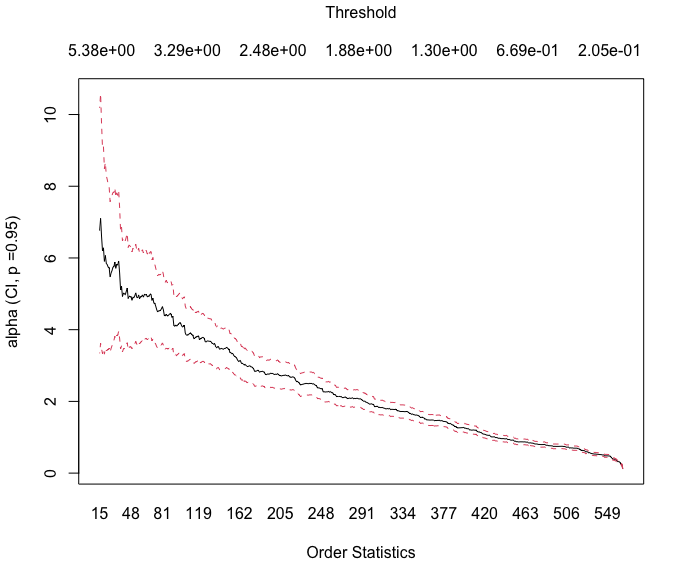
\includegraphics[width=3in]{Assignments/a3/hill-plot-ar9.png}}
\caption{Hill plot for AR(1) process with $\phi=0.9$.}
\end{center}
\end{figure}

\subsection*{$\phi=0.5$}
Although we observe more stable behavior around 10 (relative to $\phi=0.9$), we still note that the Hill plot is not stable enough around 10 to give an obvious reading. In fact, if we did not know the true underlying value of $\alpha$, we would be hard pressed to select 10 from analysis of the graph.
\begin{figure}[H]
\begin{center}
{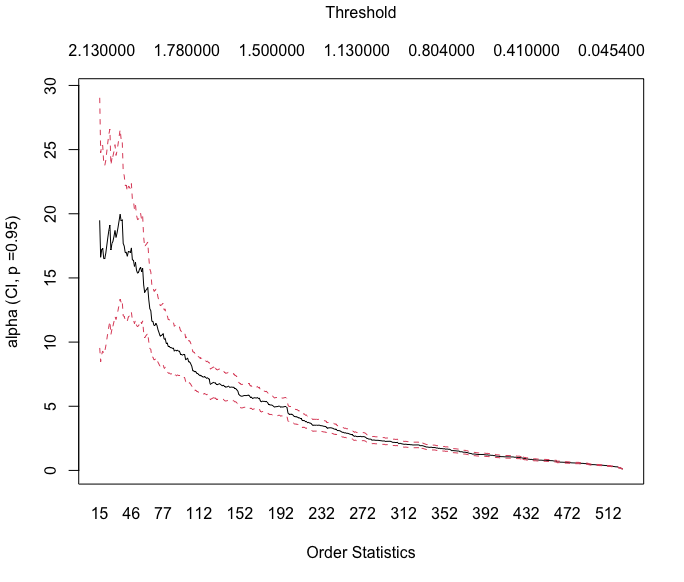
\includegraphics[width=3in]{Assignments/a3/hill-plot-ar5.png}}
\caption{Hill plot for AR(1) process with $\phi=0.5$.}
\end{center}
\end{figure}

\subsection*{$\phi=0.2$}
Here at least we see some stability. While $\hat\alpha$ seems to suggest a value around 12, this is the closest the Hill plot of our AR(1) experimental processes has gotten to the true value. However, we note that 10 is not in the confidence interval (starting from 112 ) which may suggest that the conditions on $k$ and $F$(for asymptotic normality of $\hat\alpha$) past this threshold are not satisfied.
\begin{figure}[H]
\begin{center}
{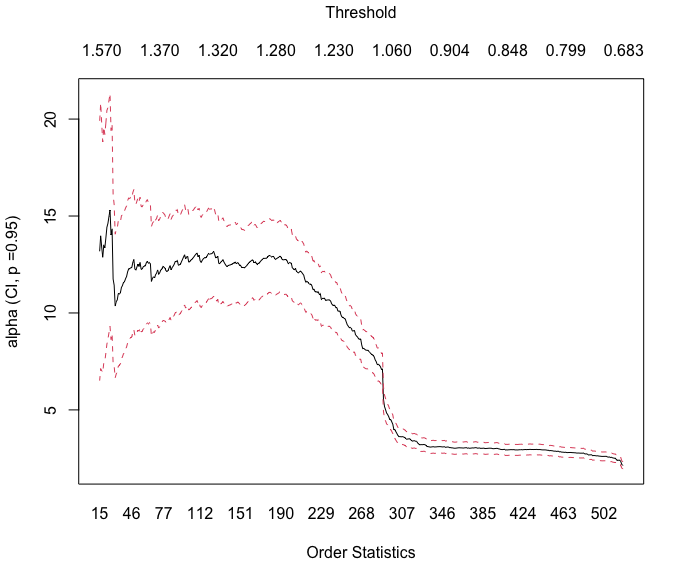
\includegraphics[width=3in]{Assignments/a3/hill-plot-ar2.png}}
\caption{Hill plot for AR(1) process with $\phi=0.2$.}
\end{center}
\end{figure}
\end{solution}

\begin{problem}{2}
We are interested in the maximum hourly rainfall in St. Louis, Missouri. The state of
Missouri suffered $\approx$ 3000 flash floods during 1996-2017, so clearly getting good estimates of the upper-tail behavior of hourly rainfall is crucial to building proper hydraulic structures and flood-protection infrastructure. 

\noindent In certain parts of the United States, rainfall is partially explained by the Southern Oscillation Index (SOI) and the Pacific Decadal Oscillation (PDO). Temperature can also partially explain precipitation. Changes over time are also possible due to climate change. Four data
files are supplied:
\begin{itemize}
    \item StLouis25.csv: hourly rainfall for months of April to August from 1979 to 2014 at a
location in St. Louis.
    \item SOIdata.csv: monthly SOI value from January 1951 to February 2020.
    \item PDOdata.csv: monthly PDO value from January 1854 to February 2020.
    \item MonthData-StLouis.csv: monthly weather statistics at St. Louis Lambert International Airport.
\end{itemize}
We focus on data for July and August. Analyzing the latter together or separately, produce useful estimates for monthly maximum hourly rainfall at this St. Louis location. Provide an executive summary of results, as well as a more detailed discussion referencing supporting
tables and figures.
\end{problem}

\begin{solution}
In our analysis, we use the supplied code to transform the hourly rainfall data into the max-monthly rainfall data. As we are looking for good estimates of the upper tail, we focus on the prediction of the $95^{th}$ and $99^{th}$ quantiles of the max rainfall data ($z_{0.05},z_{0.01}$). From our investigation, we found the best estimates to be :
\begin{align*}
    p= 0.05  && \hat{z}_{0.05}=23.67 \\
    p= 0.01  && \hat{z}_{0.01}=30.52 
\end{align*}
The methods for model creation, selection, and parameter estimation are discussed in the next sections.
\section*{Preliminary Data Analysis}
We begin our analysis by considering July and August rainfall data as one dataset. This is done to give more samples to the covariate model(s) we fit. From observation of the data (shown below) and its corresponding ACF plot, we will assume that the monthly maximum hourly rainfall data follows a process where the $D(u_n)$ condition is held. 
\begin{figure}[H]
\begin{center}
{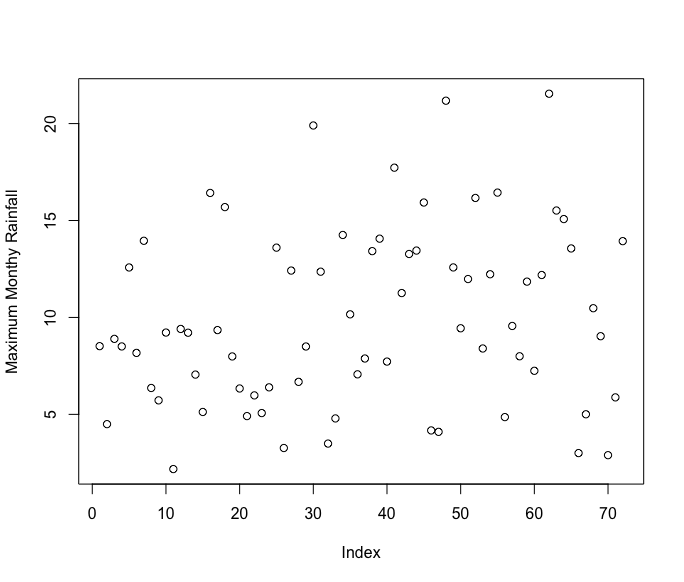
\includegraphics[width=3in]{Assignments/a3/rain.png}}
{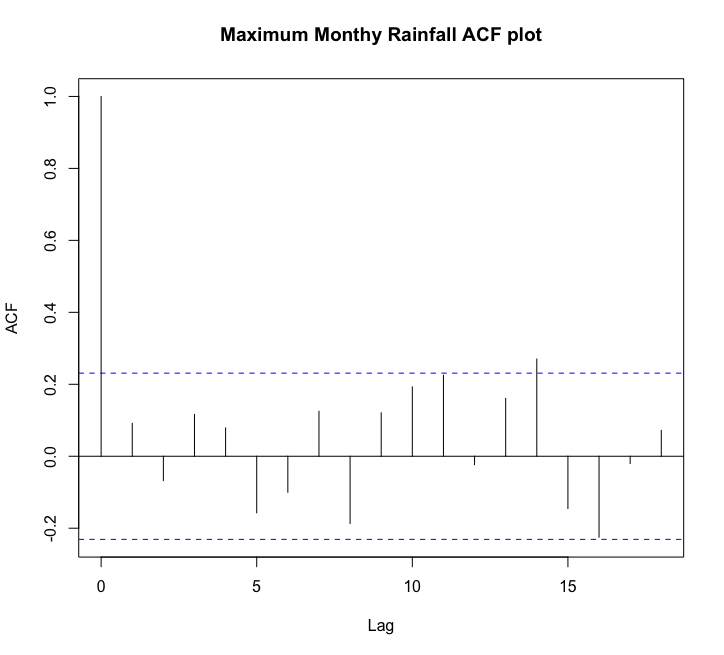
\includegraphics[width=3in]{Assignments/a3/rain-acf.png}}
\caption{Maximum monthly rain}
\end{center}
\end{figure}
\noindent This decision made, we must decide which of the supplementary data we wish to include in our model. At a later point, this will be done through model selection. However, to get an intuitive feel for the data, we plot the monthly Saint Louis data against each of these covariates in turn. From these (shown below), we note that the effects of SOI and PDO are similar with respect to the maximum monthly rainfall. This would suggest that these are affecting the same parameter (scale). However, their effects on the monthly rainfall seems to be less than the effects of the weather. We note this as the graph of rain vs weather exhibits less of an ``even" spread which may suggest that temperature affects location. Of course all of these are just speculations which we must test in our model building process.
\begin{figure}[H]
\begin{center}
{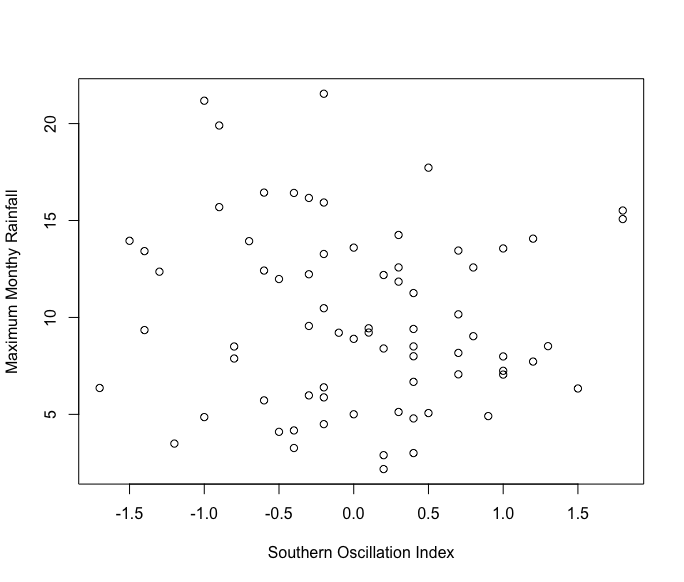
\includegraphics[width=3in]{Assignments/a3/rain-vs-soi.png}}
{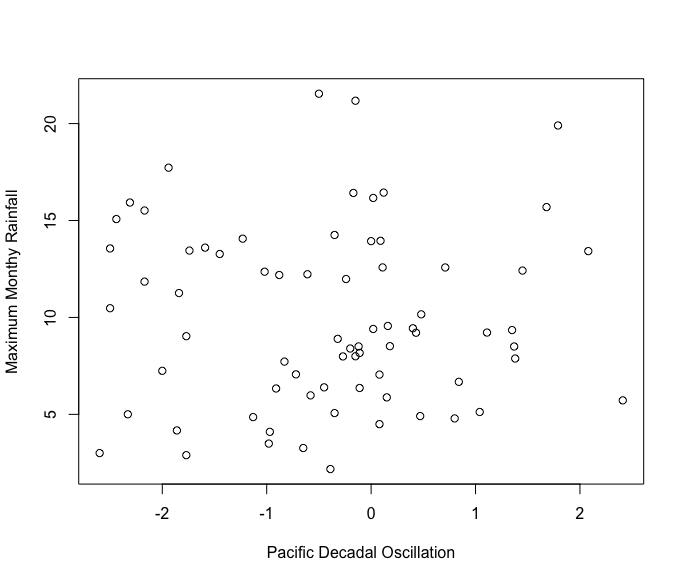
\includegraphics[width=3in]{Assignments/a3/rain-vs-pdo.png}}
{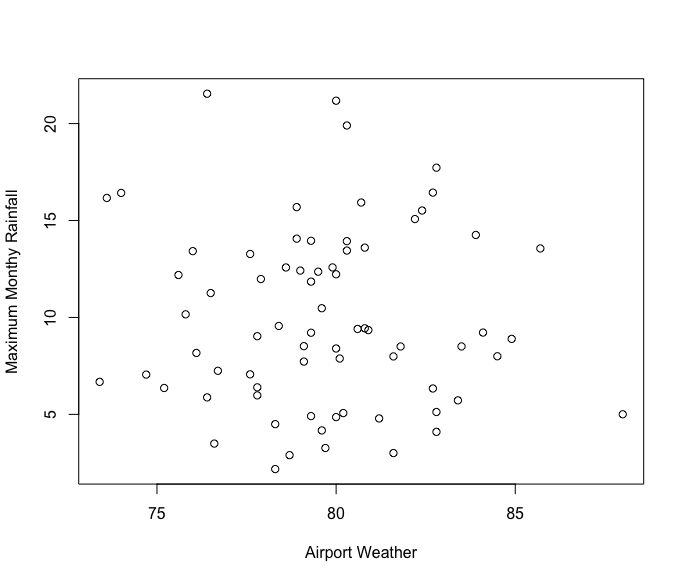
\includegraphics[width=3in]{Assignments/a3/rain-vs-temp.png}}
\caption{Maximum monthly rain plotted against potential covariates }
\end{center}
\end{figure}

\section*{Model building}
Let $\{X_t\}$ be the sequence of maximum monthly rain data. Consider the following covariate models for the location parameter:
\begin{align*}
    & \mu_3(t)=\beta_0+\beta_1\text{PDO}+\beta_2\text{SOI}+ \beta_3\text{TMP}\\
    & \mu_{2PS}(t)=\beta_0+\beta_1\text{PDO}+\beta_2\text{SOI}\\
    & \mu_{2PT}(t)=\beta_0+\beta_1\text{PDO}+\beta_2\text{TMP}\\
    & \mu_{2ST}(t)=\beta_0+\beta_1\text{SOI}+ \beta_2\text{TMP}\\
    & \mu_{1P}(t)=\beta_0+\beta_1\text{PDO}\\
    & \mu_{1S}(t)=\beta_0+\beta_1\text{SOI}\\
    & \mu_{1T}(t)=\beta_0+\beta_1\text{TMP}\\
    & \mu_0(t)=\beta_0
\end{align*}
Similarly, consider the following covariate models for the scale parameter:

\begin{align*}
    & \sigma_3(t)=\exp\{\alpha_0+\alpha_1\text{PDO}+\alpha_2\text{SOI}+ \alpha_3\text{TMP}\}\\
    & \sigma_{2PS}(t)=\exp\{\alpha_0+\alpha_1\text{PDO}+\alpha_2\text{SOI}\}\\
    & \sigma_{2PT}(t)=\exp\{\alpha_0+\alpha_1\text{PDO}+\alpha_2\text{TMP}\}\\
    & \sigma_{2ST}(t)=\exp\{\alpha_0+\alpha_1\text{SOI}+ \alpha_2\text{TMP}\}\\
    & \sigma_{1P}(t)=\exp\{\alpha_0+\alpha_1\text{PDO}\}\\
    & \sigma_{1S}(t)=\exp\{\alpha_0+\alpha_1\text{SOI}\}\\
    & \sigma_{1T}(t)=\exp\{\alpha_0+\alpha_1\text{TMP}\}\\
    & \sigma_0(t)=\alpha_0
\end{align*}
The shape parameter has been left to be modeled by a constant. To find the best model, we fit a full model
\[X_t\sim GEV(\mu_3(t),\sigma_3(t), \xi) \]
and compare it to smaller models using the deviance statistic as a guide to know if the nested models are an appropriate simplification of the more complex models. We will also be making use of the pp and qq plots to assess individual model performance. While this approach gives 64 models to test, we only need to test until we are satisfied with the number of included covariates and the diagnosis pp and qq plots. In fact, we build the full model (using $\mu_3, \sigma_3$) and prune it until removing any of the covariates drastically affects the model's predictive performance. Therefore, results from all 64 experiments are not included in this document.

\section*{Model Evaluation}
As mentioned in the previous section, we will be using quantile and probability plots to assess the performance of each model individually. Since the task is to find a good estimate for the maximum rainfall to prepare for floods, we will penalise models where the qq plot suggest the model will underestimate upper quantiles.

\noindent First, we build the model in the table below. The Deviance column refers to the deviance statistic between the model in question and the last pruned model. We say a model is stable when we fail to prune any of its covariates using hypothesis testing. Models that are kept after pruning are set in bold.
\begin{center}
    \begin{tabular}{||c||c|c|c|c||}\hline
     Model& $\mu(t)$ & $\sigma(t)$&Log Lik.& Deviance \\\hline
     I& $\mu_3$ & $\sigma_3$ & -205.99 & -- \\\hline
     \textbf{II}&$\mu_3$ & $\sigma_{2PS}$ & -205.81 & -0.372  \\\hline
     III& $\mu_3$ & $\sigma_{1S}$ & -208.03 & 4.46\\\hline
     IV& $\mu_3$ & $\sigma_{1P}$ & -208.26 & 4.91 \\\hline
\end{tabular}
\end{center}
Here we note that for a 95\% hypothesis test, we cannot reject the null hypothesis that the weather is unimportant (comparing model I and model II). However, we do see that the effects of PDO and SOI are both important as we must reject the null hypothesis when testing model II and III, and subsequently model II and IV. Next, we will do the same with the location parameter. This time, model II will serve as the base model from which we prune.

\begin{center}
    \begin{tabular}{||c||c|c|c|c||}\hline
     Model& $\mu(t)$ & $\sigma(t)$&Log Lik.& Deviance \\\hline
     II&$\mu_3$ & $\sigma_{2PS}$ & -205.81 & --  \\\hline
     V& $\mu_{2PS}$ & $\sigma_{2PS}$ & -207.97 & 4.33\\\hline
     \textbf{VI}& $\mu_{2PT}$ & $\sigma_{2PS}$ & -206.06 & 0.51 \\\hline
     \textbf{VII}& $\mu_{1T}$ & $\sigma_{2PS}$ &  -206.22 & 0.32 \\\hline
\end{tabular}
\end{center}
Here instead, we note that only the temperature has a significant effect on the location parameter. This gives rise to our final model:
\[X_t\sim GEV(\beta_0+\beta_1TMP, \exp\{\beta_0+\beta_1PDO+\beta_2SOI\}, \xi)\]
From the diagnostics pp and qq plots (below), we see that although our model is not perfect, it does an adequate job of capturing the upper quantile behavior of our data. That being said, there is some evidence that the model might under-estimate the quantiles (seen from mid-quantiles in qq plot) so an application of this model might be well served to err on the side of caution when using the estimated values of $z_p$.
\begin{figure}[H]
\begin{center}
{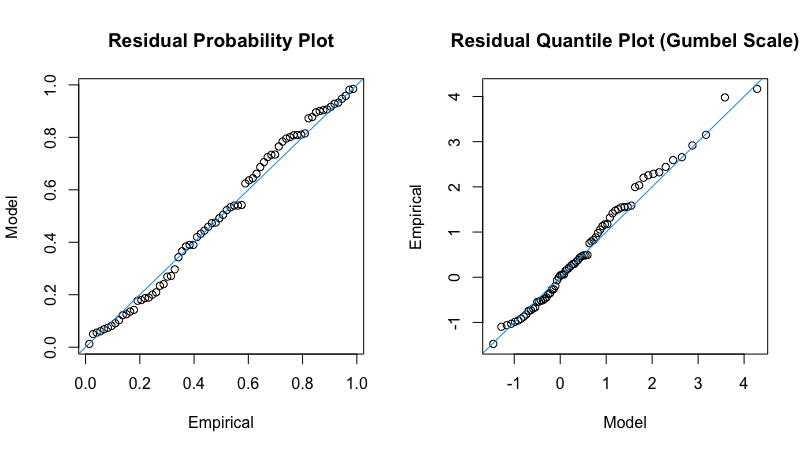
\includegraphics[width=5in]{Assignments/a3/mod7-diag.png}}
\caption{Diagnosis plots for Model VII}
\end{center}
\end{figure}
Since we used a covariate model, each of the 72 data points we have corresponds to a unique grouping of parameters $(\mu(t), \sigma(t), \xi)$. For this reason, for a given $p$, we create a list of the daily quantile $\{z_p(t)\}$ and then, use the maximum quantile in this set as our estimate. 
\[\hat{z}_p = \max_{z}\{\hat{z}_p(t)| t=1,\hdots,72\}\]

\section*{Conclusions}
From the diagnosis plot, we see that our model may under estimate the upper quantiles but it is the best model we have been able to arrive to. It is also worth mentioning that the estimate for $z_{0.01}$ is so high that it might not have any practical value since 30 is significantly larger than all previously measured hourly rainfalls in St. Louis.
\end{solution}

\end{document}

